\apendice{Documentación técnica de programación}

\section{Introducción}
Este apéndice proporciona una guía detallada sobre la estructura del código del proyecto, las herramientas usadas para el funcionamiento de la aplicación junto con su configuración.
Se analizarán la estructrura de directorios que hay en la aplicación, además se incluirá un manual del programador en el que se explicarán cómo instalar y configurar el entorno de desarrollo junto con la ejecución del proyecto.
Con este apéndice se intenta que futuros desarrolladores que vayan a modificar o mejorar la aplicación sepan como dejar todo instalado y configurado de la mejor forma posible.

\section{Estructura de directorios}

El proyecto \textbf{GreenInHouse} sigue una estructura de directorios bien organizada, permitiendo una gestión eficiente del código, los recursos y la configuración. A continuación, se describen las principales carpetas y su contenido:

\begin{itemize}
    \item {\textbf{Directorio raíz} (\texttt{greeninhouse2/})}
    Este es el directorio principal del proyecto y contiene archivos de configuración esenciales para Flutter y Dart, además de la estructura del código fuente.

    \begin{itemize}
    \item \textbf{\texttt{.dart\_tool/}}: Carpeta generada automáticamente por Flutter y Dart con herramientas internas necesarias para la compilación.
    \item \textbf{\texttt{.idea/}}: Archivos de configuración de Android Studio para la organización del proyecto.
    \item \textbf{\texttt{build/}}: Carpeta generada durante la compilación, almacena archivos de salida del proyecto.
    \item \textbf{\texttt{ios/}, \texttt{android/}, \texttt{linux/}, \texttt{macos/}, \texttt{web/}, \texttt{windows/}}: Carpetas para cada plataforma soportada, con la configuración y código necesarios para compilar en cada sistema operativo.

    \item \texttt{\textbf{assets}/} Carpeta con todas las fotos que se van a usar en la aplicación.
    \begin{itemize}
        \item \texttt{cara\_enfadada.png}
        \item \texttt{cara\_seria.png}
        \item \texttt{cara\_sonriente.png}
        \item \texttt{plant\_image.png}
    \end{itemize}
    \item \textbf{\texttt{flags/}}: Carpeta con imágenes de iconos y estados de las plantas:

    \item{\texttt{\textbf{lib/}}}
    Directorio principal del código fuente en Flutter. Aquí se encuentra la lógica de la aplicación.
    \begin{itemize}
    \item \textbf{\texttt{generated/}}: Contiene archivos generados automáticamente para la internacionalización.
    \begin{itemize}
        \item \texttt{intl/l10n.dart} – Configuración de localización.
    \end{itemize}
    \item \textbf{\texttt{l10n/}}: Dedicada a la internacionalización del proyecto.
    \begin{itemize}
        \item \texttt{intl\_en.arb} – Traducciones en inglés.
        \item \texttt{intl\_es.arb} – Traducciones en español.
    \end{itemize}

    \item \textbf{\texttt{api\_service.dart}} – Implementación de las llamadas a la API.
    \item \textbf{\texttt{botones\_inicio.dart}} – Definición de la barra de navegación inferior.
    \item \textbf{\texttt{main.dart}} – Punto de entrada principal de la aplicación.

    \item \texttt{\textbf{pantalla\_graficas.dart}} – Pantalla principal con gráficos de sensores.
    \item \texttt\textbf{{pantalla\_inicio.dart}} – Pantalla inicial de la aplicación.
    \item \texttt{\textbf{pantalla\_comprobacion\_sensores.dart}} – Revisión del estado de sensores.
    \item \texttt{\textbf{pantalla\_creacionplantas.dart}} – Creación de nuevas plantas.
    \item \texttt{\textbf{pantalla\_modificarplanta.dart}} – Modificación de plantas registradas.
    \item \texttt{\textbf{pantalla\_eliminarplanta.dart}} – Eliminación de plantas registradas.

    \item \texttt{\textbf{grafica\_humedad.dart}} – Representación de datos de humedad.
    \item \texttt{\textbf{grafica\_luz.dart}} – Visualización de datos de luminosidad.
    \item \texttt{\textbf{grafica\_temperatura.dart}} – Evolución de la temperatura.
    \end{itemize}

    \item \texttt{\textbf{.gitignore}} – Define archivos y carpetas a excluir del repositorio Git.
    \item \texttt{.metadata} – Archivo interno de configuración de Flutter.
    \item \texttt{\textbf{analysis\_options.yaml}} – Reglas de análisis de código en Dart.
    \item \texttt{\textbf{greeninhouse2.iml}} – Configuración de IntelliJ/Android Studio.
    \item \texttt{\textbf{pubspec.yaml}} – Define dependencias, assets e información del proyecto.
    \item \texttt{\textbf{pubspec.lock}} – Registro de versiones de las dependencias utilizadas.
    \item \texttt{\textbf{README.md}} – Documentación inicial sobre el proyecto y su instalación.
    \end{itemize}
\end{itemize}

\section{Manual del programador}
El objetivo del manual del programador es la de proporcionar una guía del desarrollo y mantenimiento de la aplicación. Este manual está dirigido a desarrolladores que necesiten como funciona las herramientas utilizadas en el desarrollo de esta aplicación.
También se ha incluído las instrucciones necesarias para configurar el entorno de desarrollo y ejecutar la aplicación.
Además, se ha detallado aspectos que son claves como la estructura de datos que sigue la aplicación y la comunicación con la API entre otras cosas con el objetivo de facilitar mejoras que se puedan llevar a cabo en un futuro.


\subsection{\textbf{Instalación de Android Studio}}
Android Studio es el entorno de desarrollo integrado (IDE) oficial que se usa en el desarrollo de apps para Android. Basado en el potente editor de código y las herramientas para desarrolladores de IntelliJ IDEA.
Se puede descargar desde su página oficial: https://developer.android.com/studio?hl=es-419



\begin{figure}[H]
    \centering
    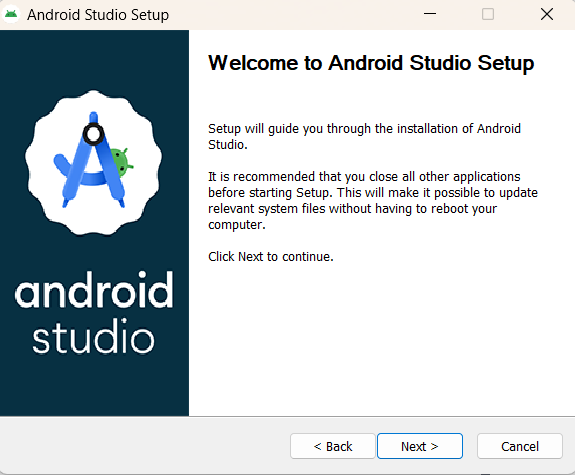
\includegraphics[width=0.8\linewidth]{AndroidStudio1.png}
    \caption{Al descargar la aplicación y ejecutarla nos saldrá lo que vemos en la foto a continuación y le daremos al botón de "Next".}
    \label{fig:enter-label}
\end{figure}



\begin{figure}[H]
    \centering
    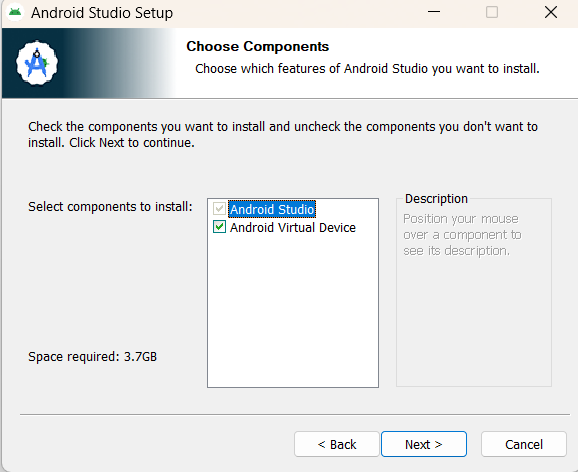
\includegraphics[width=0.8\linewidth]{AndroidStudio2.png}
    \caption{Tras esto nos saldrá la siguiente ventana en la que dejaremos lo que viene por defecto y le volveremos a dar a "Next".}
    \label{fig:enter-label}
\end{figure}


\begin{figure}[H]
    \centering
    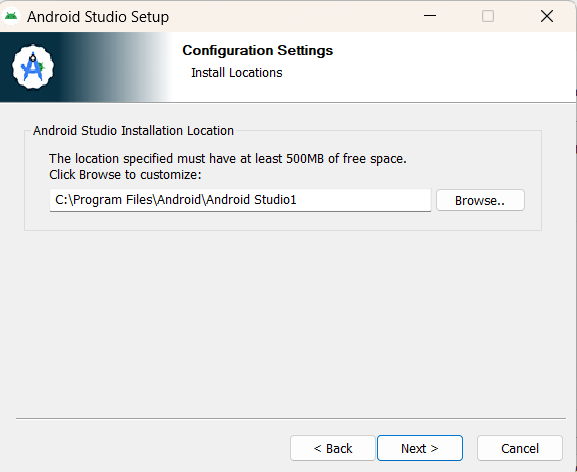
\includegraphics[width=0.8\linewidth]{AndroidStudio3.png}
    \caption{Por último en la ultima ventana decidiremos el path donde instalar la aplicación y le daremos a "Next" para que instale la aplicación en el path seleccionado.}
    \label{fig:enter-label}
\end{figure}

Tras instalar Android Studio vamos a pasar a la configuración de las herramientas instalando tanto Flutter como Dart.
Esto se hace entrando en la pestaña de ajustes y en Plugins.

\begin{figure}[H]
    \centering
    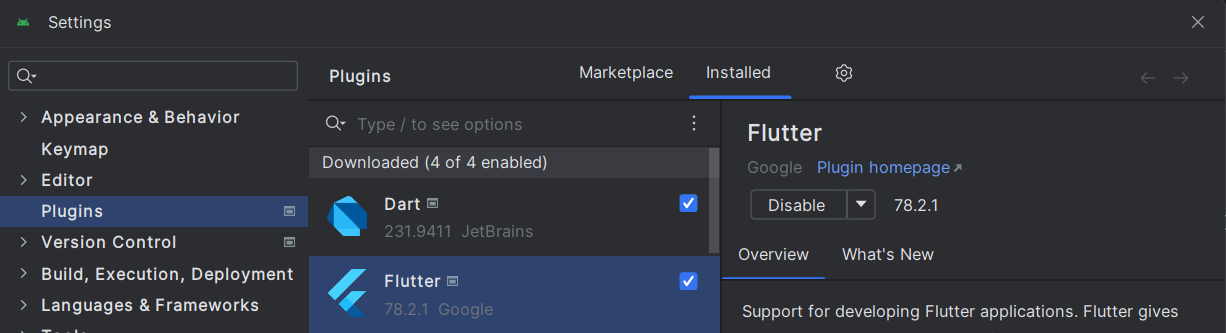
\includegraphics[width=0.8\linewidth]{PlugingsAndroidStudio.png}
    \caption{Instalación plugins Android Studio}
    \label{fig:enter-label}
\end{figure}


El siguiente paso es la configuración de SDK en el Android Studio. Esto se hace accediendo a ajustes y alli desde Languages \& Frameworks.

\begin{figure}[H]
    \centering
    \includegraphics[width=0.8\linewidth]{Configuración-SDK-AndroidStudio.png}
    \caption{Configuración de SDK en Android Studio}
    \label{fig:enter-label}
\end{figure}


Por ultimo vamos a instalar unas herramientas en SDK Tools que viene a la derecha de la de SDK Platforms necesarias para el buen funcionamiento de la herramienta.

\begin{figure}[H]
    \centering
    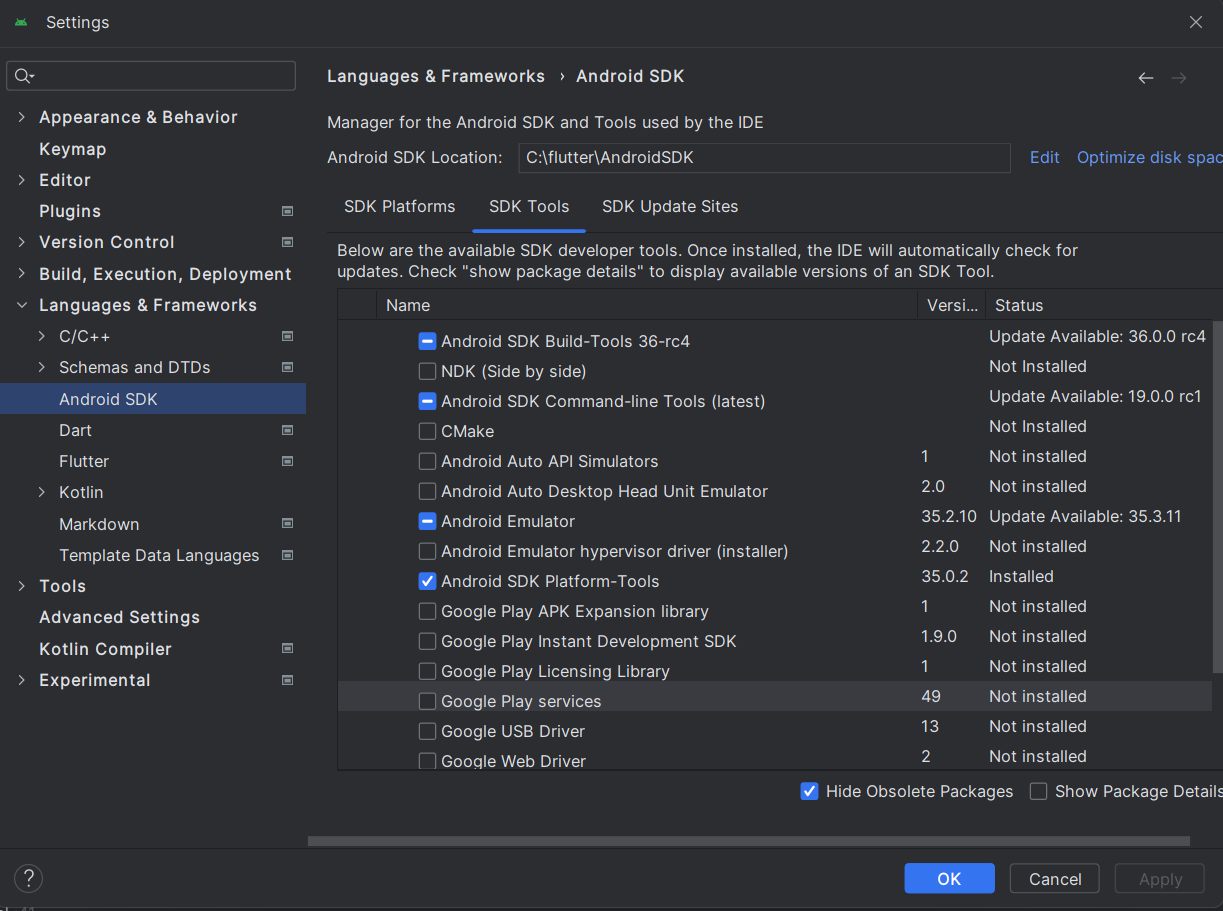
\includegraphics[width=0.8\linewidth]{Configuracion-SDKTools-AndroidStudio.png}
    \caption{Instalación de Herramientas de SDK}
    \label{fig:enter-label}
\end{figure}

\subsection{\textbf{Instalación de Flutter}}

\section{Compilación, instalación y ejecución del proyecto}

\section{Pruebas del sistema}
